\documentclass[a4paper,11pt]{article}

% ---------- Encoding & Fonts ----------
\usepackage[T1]{fontenc}
\usepackage[utf8]{inputenc}
\usepackage{lmodern}       % clean Latin Modern font
\usepackage{microtype}     % better kerning/justification

% ---------- Geometry & Layout ----------
\usepackage[top=27mm, bottom=30mm, left=26mm, right=26mm]{geometry}
\setlength{\parskip}{6pt}
\setlength{\parindent}{0pt} % unindented paragraphs (toggle if you prefer)

% ---------- Math & Figures ----------
\usepackage{amsmath, amssymb, amsfonts}
\usepackage{graphicx}
\usepackage{booktabs}      % nice tables

\usepackage{caption}
\captionsetup{labelfont=bf, font=small, labelsep=period}
\usepackage{subcaption}
\usepackage{float}     % Görsel pozisyonu için [H] kullanmak istersen
% ---------- Diagrams ----------
\usepackage{standalone}
\usepackage{tikz}
\usepackage{helvet}
\usetikzlibrary{shapes.geometric, arrows, positioning, fit, backgrounds, calc}
% Styles for architecture diagram
\tikzstyle{databox} = [rectangle, rounded corners, minimum width=3cm, minimum height=1.2cm, align=center, draw=blue!70, fill=blue!15, thick, font=\small]
\tikzstyle{frozenbox} = [rectangle, rounded corners, minimum width=2.8cm, minimum height=1cm, align=center, draw=red!70, fill=red!10, thick, font=\footnotesize]
\tikzstyle{trainablebox} = [rectangle, rounded corners, minimum width=2.8cm, minimum height=1cm, align=center, draw=blue!80, fill=blue!25, thick, font=\footnotesize]
\tikzstyle{processbox} = [rectangle, rounded corners, minimum width=2.5cm, minimum height=0.9cm, align=center, draw=gray!70, fill=gray!10, thick, font=\footnotesize]
\tikzstyle{unetbox} = [rectangle, rounded corners, minimum width=3.5cm, minimum height=3cm, align=center, draw=red!70, fill=red!8, thick, font=\footnotesize]
\tikzstyle{configbox} = [rectangle, rounded corners, minimum width=4cm, minimum height=2.5cm, align=left, draw=green!70, fill=green!10, thick, font=\scriptsize]
\tikzstyle{inferencebox} = [rectangle, rounded corners, minimum width=14cm, minimum height=1.5cm, align=center, draw=purple!70, fill=purple!8, thick, font=\footnotesize]
\tikzstyle{outputbox} = [rectangle, rounded corners, minimum width=2.8cm, minimum height=0.8cm, align=center, draw=green!60, fill=green!5, thick, font=\scriptsize]
\tikzstyle{imagebox} = [rectangle, minimum width=1.5cm, minimum height=1.5cm, draw=black!50, fill=white, thick]
\tikzstyle{arrow} = [thick,->,>=stealth, line width=0.8pt]
\tikzstyle{dashedarrow} = [thick,->,>=stealth,dashed,blue!70, line width=1pt]
\tikzstyle{groupbox} = [rectangle, rounded corners, draw, thick, inner sep=8pt]
% ---------- Lists & Quotes ----------
\usepackage{enumitem}
\setlist{nosep}
\usepackage{csquotes}

% ---------- Links ----------
\usepackage[hidelinks]{hyperref}
\usepackage{cleveref} % must be loaded after hyperref
\hypersetup{
  pdftitle={Mask2Derm: Photorealistic and Controllable Skin Lesion Synthesis via Latent Diffusion},
  pdfauthor={Can Rollas et al.},
  pdfkeywords={dermoscopy, ControlNet, diffusion, augmentation},
  pdfstartview=FitH 
}

% ---------- Bibliography ----------
% \usepackage[backend=biber, style=numeric, sorting=none, maxnames=15, giveninits=true]{biblatex}
% \addbibresource{references.bib}
% ---------- Header / Footer ----------
\usepackage{fancyhdr}
\pagestyle{fancy}
\fancyhf{}
% Define short title & authors for running heads
\newcommand{\shorttitle}{Mask2Derm: Photorealistic and Controllable Skin Lesion Synthesis}
\newcommand{\shortauthors}{Can Rollas et al.}
\fancyhead[LE]{\thepage \quad \shortauthors}
\fancyhead[RO]{\shorttitle \quad \thepage}
\renewcommand{\headrulewidth}{0.4pt}

% ---------- Section Titles ----------
\usepackage{titlesec}
\titleformat{\section}{\large\bfseries}{\thesection}{0.6em}{}
\titleformat{\subsection}{\normalsize\bfseries}{\thesubsection}{0.6em}{}
\titleformat{\subsubsection}{\normalsize\itshape}{\thesubsubsection}{0.6em}{}

% ---------- Author & Affiliation ----------
\usepackage{authblk}
\renewcommand\Authfont{\large\bfseries}
\renewcommand\Affilfont{\normalsize\normalfont}
\setlength{\affilsep}{0.5em}

% ---------- Abstract Box ----------
\usepackage[most]{tcolorbox}
\tcbset{
  enhanced,
  colback=white,
  colframe=black!10,
  boxrule=0.5pt,
  arc=2pt,
  left=8pt,right=8pt,top=6pt,bottom=6pt
}
\newenvironment{boxedabstract}
{\begin{tcolorbox}\textbf{Abstract.}\ }
{\end{tcolorbox}}

% ---------- Custom Blocks ----------
\newenvironment{contributions}{\par\noindent\textbf{Contributions.}\ }{\par}
\newenvironment{keywordsblock}{\par\noindent\textbf{Keywords.}\ }{\par}

% Optional: line numbers for review (toggle on/off)
% \usepackage[displaymath, mathlines]{lineno}
% \linenumbers

% =========================================================
%                         Document 
% =========================================================
\begin{document}

\title{\vspace{-6mm}\Large Mask2Derm: Photorealistic and Controllable Skin Lesion Synthesis via Latent Diffusion}
\author[1,2]{Can Rollas\thanks{Corresponding author: \texttt{c.rollas@amatis.nl}}}
\author[1,3]{Mehmet Kemal Güllü}
\author[1,4]{İbrahim Onur Alıcı}

\affil[1]{R\&D Department, Amatis IT, \url{www.amatis.nl}}
\affil[2]{Department of Computer Engineering, Faculty of Engineering, Izmir Institute of Technology (IZTECH)}
\affil[3]{Department of Electrical and Electronics Engineering, Faculty of Engineering and Architecture, İzmir Bakırçay University}
\affil[4]{Department of Biomedical Engineering, Faculty of Engineering and Architecture, İzmir Bakırçay University}

\date{} % no date
\maketitle

\begin{boxedabstract}
Despite rapid advances in computer vision and generative AI, data sharing and the lack of standardized datasets remain major bottlenecks in medical imaging. We consolidate multiple public dermoscopy sources into a harmonized 11k-image corpus with consistent labels and resolutions. On this corpus, we train a ControlNet-based latent diffusion model conditioned solely on a user-provided lesion segmentation mask. Given a fixed-size (binary) mask, our method synthesizes photorealistic dermoscopic images that faithfully conform to the input shape. Quantitative evaluation reveals a high shape consistency (Dice: 0.92, IoU: 0.87). Crucially, in a Train-on-Synthetic, Test-on-Real (TSTR) benchmark, a segmentation model trained solely on our synthetic data outperformed an ImageNet-initialized baseline by 13.4\% in IoU (0.93 vs 0.79), validating the clinical utility of the generated corpus.  
\end{boxedabstract}

\begin{keywordsblock}
Dermoscopy, ControlNet, Diffusion Models, Data Augmentation
\end{keywordsblock}

\vspace{2mm}
\begin{contributions}
A ControlNet-driven mask-to-image pipeline.
\end{contributions}

% ---------------------------
\section*{Introduction}
Skin cancer is a common skin disease whose incidence and mortality rates have been showing increases yearly~\cite{Wang_M}. Despite rapid progress in deep learning for dermoscopic analysis, model performance and robustness are still bounded by data scarcity, curation costs, and the heterogeneity of imaging devices and acquisition protocols. Public dermoscopy datasets exist, yet they vary in resolution, color calibration, annotation quality, and class balance, which complicates training and reproducibility. In this work, we address these limitations by (i) unifying multiple public dermoscopy sources, including ISIC-2018~\cite{Codella2019ISIC2018} and HAM10000~\cite{Tschandl2018HAM10000}, into a standardized collection of approximately 11,000 images with consistent preprocessing and mask formats, and (ii) introducing a diffusion-based generation pipeline conditioned on segmentation masks via ControlNet~\cite{zhang2023adding}. Our goal is to synthesize \emph{photorealistic} dermoscopic images that respect lesion geometry (shape, borders, and asymmetries) while enriching appearance diversity (pigment networks, streaks, regression structures) in a controllable manner. The pipeline can produce realistic variants for rare patterns and device domains, supporting both data augmentation and stress-testing for downstream tasks. Our work contributes to a growing field of generative synthesis for dermoscopy. While earlier works utilized Generative Adversarial Networks (GANs) to address class imbalance~\cite{qasim2021redganattackingclassimbalance}, recent efforts have shifted towards diffusion models for tasks such as boosting segmentation performance~\cite{du2023boostingdermatoscopiclesionsegmentation} or performing dual-task and simultaneous image-mask generation~\cite{SheJun_DiDGen_MICCAI2025, xu2025skindualgenpromptdrivendiffusionsimultaneous}.

% ===== TEMEL KULLANIM =====
Our image synthesis pipeline is built upon the latent diffusion model framework~\cite{Rombach2022LDM}, utilizing the pre-trained Realistic Vision V5.1 as its backbone. As illustrated in Figure~\ref{fig:architecture}, this foundational model consists of three core components: (i) a Variational Autoencoder (VAE), (ii) a U-Net based denoiser, and (iii) a CLIP text encoder.

\begin{figure}[H]
    \centering
    \resizebox{\linewidth}{!}{%
        \sffamily
        \documentclass{standalone}
\usepackage[utf8]{inputenc}
\usepackage{tikz}
\usetikzlibrary{shapes.geometric, arrows, positioning, fit, backgrounds, calc, matrix}
\usepackage{helvet}
\renewcommand{\familydefault}{\sfdefault}

% Colors are still useful in preamble for standalone, but we'll use literal colors or re-define them if needed in main.
% To be safe, we use standard colors in the styles below or define them in the tikzpicture scope if they are custom.
% Defining them globally in the doc body is safest for input.

\definecolor{frozen}{RGB}{200, 200, 200}
\definecolor{trainable}{RGB}{255, 150, 100}
\definecolor{data}{RGB}{100, 180, 255}
\definecolor{process}{RGB}{220, 220, 250}

\begin{document}
% We embed styles here so they are preserved when imported via \input into main.tex
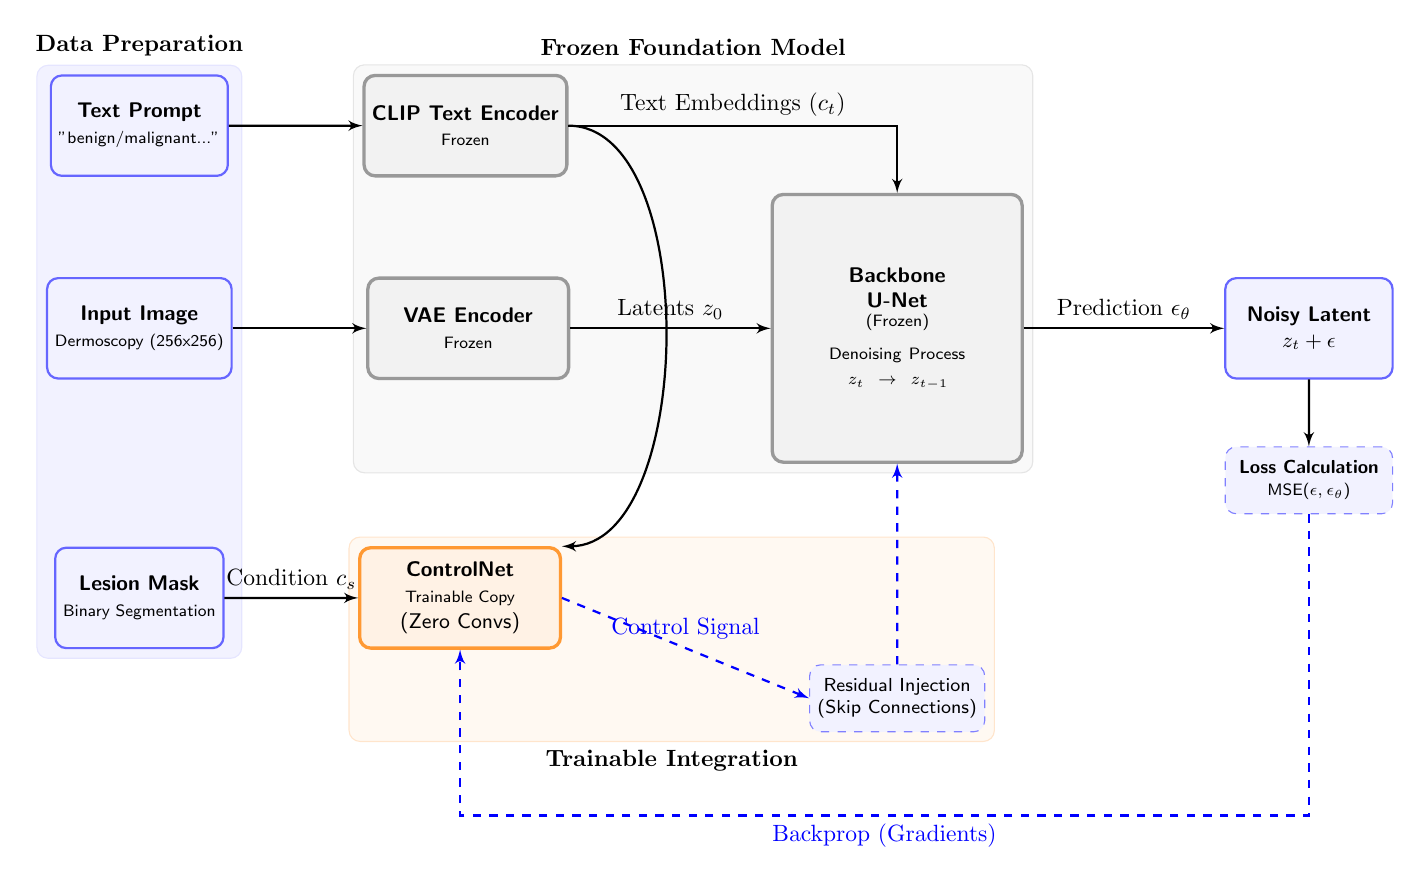
\begin{tikzpicture}[
    node distance=2.5cm, 
    auto, 
    scale=0.85, 
    transform shape, 
    ampersand replacement=\&,
    % Styles embedded for portability
    box_frozen/.style={rectangle, rounded corners, minimum width=3cm, minimum height=1.5cm, align=center, draw=gray!80, fill=gray!10, very thick, font=\sffamily\small},
    box_trainable/.style={rectangle, rounded corners, minimum width=3cm, minimum height=1.5cm, align=center, draw=orange!80, fill=orange!10, very thick, font=\sffamily\small},
    box_data/.style={rectangle, rounded corners, minimum width=2.5cm, minimum height=1.5cm, align=center, draw=blue!60, fill=blue!5, thick, font=\sffamily\small},
    process/.style={rectangle, rounded corners, minimum width=2.5cm, minimum height=1cm, align=center, draw=blue!50, fill=blue!5, dashed, font=\sffamily\footnotesize},
    line/.style={draw, -latex', thick},
    dashedline/.style={draw, -latex', dashed, thick, blue}
]

    % --- LAYER 1: DATA INPUTS (Left Side) ---
    \node [box_data] (img) {\textbf{Input Image}\\\scriptsize Dermoscopy (256x256)};
    \node [box_data, below=2.5cm of img] (mask) {\textbf{Lesion Mask}\\\scriptsize Binary Segmentation};
    \node [box_data, above=1.5cm of img] (prompt) {\textbf{Text Prompt}\\\scriptsize "benign/malignant..."};

    % --- LAYER 2: ENCODERS (Column 2) ---
    \node [box_frozen, right=2cm of img] (vae) {\textbf{VAE Encoder}\\\scriptsize Frozen};
    \node [box_trainable, right=2cm of mask] (controlnet) {\textbf{ControlNet}\\\scriptsize Trainable Copy\\(Zero Convs)};
    \node [box_frozen, right=2cm of prompt] (clip) {\textbf{CLIP Text Encoder}\\\scriptsize Frozen};

    % --- LAYER 3: DIFFUSION PROCESS (Column 3) ---
    % UNet is the core, sits in the middle
    \node [box_frozen, right=3cm of vae, minimum height=4cm, text width=3.5cm] (unet) {\textbf{Backbone}\\\textbf{U-Net}\\\scriptsize (Frozen)\\\vspace{0.2cm}Denoising Process\\$z_t \rightarrow z_{t-1}$};
    
    % Control Signal Injection
    \node [process, below=of unet, yshift=-0.5cm] (injection) {Residual Injection\\(Skip Connections)};

    % --- LAYER 4: OUTPUT & LOSS (Far Right) ---
    \node [box_data, right=3cm of unet] (output) {\textbf{Noisy Latent}\\$z_t + \epsilon$};
    \node [process, below=1cm of output] (loss) {\textbf{Loss Calculation}\\\scriptsize MSE($\epsilon, \epsilon_\theta$)};
    
    % --- CONNECTIONS ---
    
    % Text Flow
    \draw [line] (prompt) -- (clip);
    \draw [line] (clip) -| node[near start, above] {Text Embeddings ($c_t$)} (unet.north);
    \draw [line] (clip.east) .. controls +(2,0) and +(2,0) .. (controlnet.north east);

    % Image Flow
    \draw [line] (img) -- (vae);
    \draw [line] (vae) -- node[above] {Latents $z_0$} (unet);

    % Control Flow
    \draw [line] (mask) -- node[above] {Condition $c_s$} (controlnet);
    % Route through Injection Node
    \draw [dashedline] (controlnet.east) -- node[above] {Control Signal} (injection.west);
    \draw [dashedline] (injection.north) -- (unet.south);
    
    % Training Loop (Symbolic)
    \draw [line] (unet) -- node[above] {Prediction $\epsilon_\theta$} (output);
    \draw [line] (output) -- (loss);
    % Reroute backprop to go under everything
    \draw [dashedline] (loss.south) -- ++(0,-4.5cm) -| node[near start, below] {Backprop (Gradients)} (controlnet.south);

    % --- GROUPING & BACKGROUNDS ---
    \begin{scope}[on background layer]
        % Blue Zone: Data Preparation
        \node [fill=blue!5, fit=(img) (mask) (prompt), rounded corners, draw=blue!10, label=above:\textbf{Data Preparation}] (prep_zone) {};
        
        % Gray Zone: Pretrained Frozen Model
        \node [fill=gray!5, fit=(clip) (vae) (unet), rounded corners, draw=gray!20, label=above:\textbf{Frozen Foundation Model}] (frozen_zone) {};
        
        % Orange Zone: Trainable Parts
        \node [fill=orange!5, fit=(controlnet) (injection), rounded corners, draw=orange!20, label=below:\textbf{Trainable Integration}] (train_zone) {};
    \end{scope}

\end{tikzpicture}
\end{document}
%
    }
    \caption{General architecture of the proposed Mask-Conditioned ControlNet pipeline.}
    \label{fig:architecture}
\end{figure}

The specific innovation lies in the integration of the ControlNet module. To prevent the collapse of pre-trained priors during fine-tuning, ControlNet employs "zero convolution" layers---$1\times1$ convolutions initialized with both weights and biases at zeros. Let $\mathcal{F}(x; \Theta)$ represent a neural network block. The ControlNet locks the original parameters $\Theta$ and creates a trainable copy $\Theta_c$. The connection is governed by two zero convolution layers $\mathcal{Z}(\cdot; \Theta_{z1})$ and $\mathcal{Z}(\cdot; \Theta_{z2})$:
\begin{equation}
    y_c = \mathcal{F}(x; \Theta) + \mathcal{Z}(\mathcal{F}(x + \mathcal{Z}(c; \Theta_{z1}); \Theta_c); \Theta_{z2})
\end{equation}
where $y_c$ is the output of the ControlNet block and $c$ is the segmentation mask condition. This formulation follows the standard ControlNet residual injection mechanism without architectural modification. Because the zero convolutions are initialized to zero, at the start of training ($y_c = \mathcal{F}(x; \Theta)$), the model behaves exactly like the original pre-trained backbone. This allows the spatial conditioning to be learned progressively without disrupting the original generative capabilities.

The training objective is consistent with standard diffusion models. The model is optimized by minimizing the mean squared error (MSE)... 


% ---------------------------
\section{Methodology}\label{sec:method}

In this section, we present the proposed pipeline for photorealistic and controllable skin lesion synthesis. The overall workflow, illustrated in Figure~\ref{fig:pipeline}, follows a sequential generation process: (1) specification of the lesion geometry via a mask, (2) conditioning of the diffusion model via ControlNet, and (3) final image synthesis.

\begin{figure}[H]
    \centering
    \resizebox{\linewidth}{!}{\documentclass{standalone}
\usepackage[utf8]{inputenc}
\usepackage{tikz}
\usetikzlibrary{shapes.geometric, arrows, positioning, fit, backgrounds, calc}
\usepackage{helvet}
\renewcommand{\familydefault}{\sfdefault}

\begin{document}
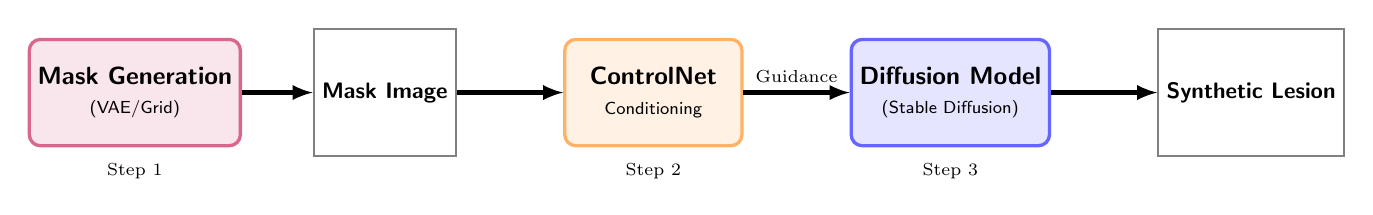
\begin{tikzpicture}[
    node distance=1.5cm,
    auto,
    scale=0.9,
    transform shape,
    box/.style={rectangle, rounded corners, minimum width=2.5cm, minimum height=1.5cm, align=center, draw=black!70, very thick, font=\sffamily},
    maskstep/.style={box, fill=purple!10, draw=purple!60},
    controlstep/.style={box, fill=orange!10, draw=orange!60},
    genstep/.style={box, fill=blue!10, draw=blue!60},
    image/.style={rectangle, minimum size=1.8cm, align=center, draw=black!50, fill=white, thick, font=\sffamily\small},
    arrow/.style={-latex, thick, line width=1.5pt}
]

    % Step 1: Mask
    \node[maskstep] (mask_gen) {\textbf{Mask Generation}\\\scriptsize (VAE/Grid)};
    \node[image, right=1cm of mask_gen] (mask_img) {\textbf{Mask Image}};
    
    % Step 2: ControlNet
    \node[controlstep, right=1.5cm of mask_img] (controlnet) {\textbf{ControlNet}\\\scriptsize Conditioning};
    
    % Step 3: Generation
    \node[genstep, right=1.5cm of controlnet] (diffusion) {\textbf{Diffusion Model}\\\scriptsize (Stable Diffusion)};
    
    % Output
    \node[image, right=1.5cm of diffusion] (output) {\textbf{Synthetic Lesion}};

    % Connections
    \draw[arrow] (mask_gen) -- (mask_img);
    \draw[arrow] (mask_img) -- (controlnet);
    \draw[arrow] (controlnet) -- node[above] {\scriptsize Guidance} (diffusion);
    \draw[arrow] (diffusion) -- (output);
    
    % Annotations
    \node[below=0.1cm of mask_gen] {\scriptsize Step 1};
    \node[below=0.1cm of controlnet] {\scriptsize Step 2};
    \node[below=0.1cm of diffusion] {\scriptsize Step 3};

\end{tikzpicture}
\end{document}
}
    \caption{Overview of the Mask2Derm pipeline: Proceeding from mask generation to ControlNet conditioning and final lesion synthesis.}
    \label{fig:pipeline}
\end{figure}

We first detail the physics-based data standardization process designed to unify heterogeneous sources. Subsequently, we describe the Mask-Conditioned ControlNet architecture and the training strategy. Finally, we outline the evaluation protocols used to assess fidelity and realism.

\subsection{Optics-Inspired Data Standardization}
To harmonize the heterogeneous dermoscopy images into a consistent optical format, we implemented an optics-inspired simulation pipeline that models the characteristics of a dermatoscope. This process integrates three optical effects: a circular field-of-view, optical vignetting, and radial lens distortion.

First, we define the radial distance $d(x, y) = \sqrt{(x - c_x)^2 + (y - c_y)^2}$ from the image center $(c_x, c_y)$. This distance map drives both the circular aperture mask $M(d)$ and the vignetting falloff $V(d)$:
\begin{equation}
    M(d) = \begin{cases} 
    1, & d \leq R \\
    \text{smooth}, & R < d \leq R + \delta \\
    0, & d > R + \delta
    \end{cases}
    \quad \text{and} \quad
    V(d) = (1 - \alpha) + \alpha \left( 1 - (d/R)^2 \right)^\gamma
\end{equation}
where $R$ is the aperture radius, $\delta$ is the feathering margin, $\alpha$ controls vignetting strength, and $\gamma$ governs the falloff rate.

Simultaneously, we simulate barrel distortion by warping the coordinates. The distorted coordinates $(x_d, y_d)$ are computed via a radial displacement model:
\begin{align}
    X &= \frac{x - c_x}{f_x}, \quad Y = \frac{y - c_y}{f_y}, \quad r^2 = X^2 + Y^2 \nonumber \\
    x_d &= f_x X(1 + k_1 r^2) + c_x, \quad y_d = f_y Y(1 + k_1 r^2) + c_y
\end{align}
where $k_1 < 0$ induces the barrel effect. The final simulated image $I'(x, y)$ combines these components: $I'(x, y) = I(x_d, y_d) \cdot M(d) \cdot V(d)$.

\begin{figure}[H]
    \centering
    \includegraphics[width=0.6\linewidth]{lens_simulation_comparison.png}
    \caption{A visual comparison of a dermoscopic image before (left) and after (right) applying the physics-based circular lens simulation.}
    \label{fig:lens_sim}
\end{figure}

After completing this standardization process, each processed image and lesion mask were used as a training pair. This ensures the model learns to generate synthetic images that conform to the mask while possessing consistent optical features.

\subsection{Mask-Conditioned ControlNet}

Our image synthesis pipeline is built upon the latent diffusion model framework, specifically using the pre-trained Realistic Vision V5.1 as its backbone. We treat Realistic Vision purely as a frozen image prior, analogous to Stable Diffusion v1.5 fine-tuning practices. This foundational model consists of three core components: (i) a Variational Autoencoder (VAE) that encodes images from pixel space into a lower-dimensional latent space and decodes them back, (ii) a U-Net based denoiser that operates in this latent space, and (iii) a CLIP text encoder that provides textual conditioning. To enable precise geometric control based on segmentation masks, we integrate a ControlNet module pre-trained for segmentation tasks.

The VAE architecture, depicted in Figure~\ref{fig:vae}, is critical for computational efficiency. It compresses high-resolution images into a lower-dimensional latent space, allowing the diffusion process to operate on significantly smaller tensors without losing semantic detail.

\begin{figure}[H]
    \centering
    \resizebox{\linewidth}{!}{\documentclass{standalone}
\usepackage[utf8]{inputenc}
\usepackage{tikz}
\usetikzlibrary{shapes.geometric, arrows, positioning, fit, backgrounds, calc}
\usepackage{helvet}
\renewcommand{\familydefault}{\sfdefault}

\begin{document}
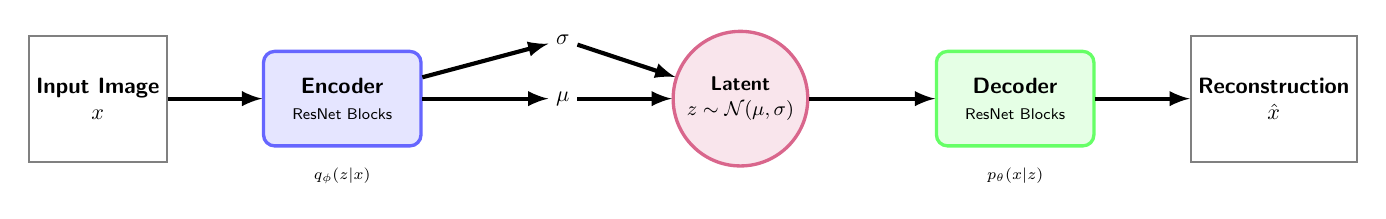
\begin{tikzpicture}[
    node distance=2cm,
    auto,
    scale=0.8,
    transform shape,
    box/.style={rectangle, rounded corners, minimum width=2.5cm, minimum height=1.5cm, align=center, draw=black!70, very thick, font=\sffamily},
    enc/.style={box, fill=blue!10, draw=blue!60},
    dec/.style={box, fill=green!10, draw=green!60},
    latent/.style={circle, minimum size=1.5cm, align=center, draw=purple!60, fill=purple!10, very thick, font=\sffamily\small},
    image/.style={rectangle, minimum size=2cm, align=center, draw=black!50, fill=white, thick, font=\sffamily},
    arrow/.style={-latex, thick, line width=1.5pt}
]

    % Input Image
    \node[image] (input) {\textbf{Input Image}\\$x$};

    % Encoder
    \node[enc, right=1.5cm of input] (encoder) {\textbf{Encoder}\\\scriptsize ResNet Blocks};
    
    % Latent Distribution
    \node[right=2cm of encoder] (mu) {$\mu$};
    \node[above=0.5cm of mu] (sigma) {$\sigma$};
    \node[latent, right=1.5cm of mu] (z) {\textbf{Latent}\\$z \sim \mathcal{N}(\mu, \sigma)$};
    
    % Decoder
    \node[dec, right=2cm of z] (decoder) {\textbf{Decoder}\\\scriptsize ResNet Blocks};
    
    % Output Image
    \node[image, right=1.5cm of decoder] (output) {\textbf{Reconstruction}\\$\hat{x}$};

    % Connections
    \draw[arrow] (input) -- (encoder);
    \draw[arrow] (encoder) -- node[above] {} (mu);
    \draw[arrow] (encoder) -- (sigma);
    \draw[arrow] (mu) -- (z);
    \draw[arrow] (sigma) -- (z);
    \draw[arrow] (z) -- (decoder);
    \draw[arrow] (decoder) -- (output);
    
    % Annotations
    \node[below=0.2cm of encoder] {\scriptsize $q_\phi(z|x)$};
    \node[below=0.2cm of decoder] {\scriptsize $p_\theta(x|z)$};

\end{tikzpicture}
\end{document}
}
    \caption{VAE Architecture: The input image is encoded into a latent distribution $z$, from which the reconstructed image $\hat{x}$ is decoded. The diffusion process operates within this compressed latent space.}
    \label{fig:vae}
\end{figure}

The key principle of this architecture is to keep the powerful, pre-trained weights of the foundation model frozen, ensuring that its rich generative priors are preserved. The ControlNet module acts as a trainable conditioning pathway. It creates a trainable copy of the U-Net's encoder blocks and middle block. During training, this copy receives the segmentation mask as an additional spatial condition and processes it in parallel with the standard denoising U-Net. The outputs of the ControlNet's blocks are then fed as residual additions to the corresponding decoder blocks of the frozen U-Net. This mechanism injects the spatial information from the mask directly into the generation process, forcing the synthesized image to conform to the input shape without catastrophic forgetting or the need to retrain the entire backbone.

The training objective is consistent with standard diffusion models. The model is optimized by minimizing the mean squared error (MSE) between the noise predicted by the U-Net and the actual noise that was initially added to the latent representation of the training image. Formally, the loss $\mathcal{L}$ is defined as:
\[
\mathcal{L} = \mathbb{E}_{\mathbf{x}_0, \boldsymbol{\epsilon} \sim \mathcal{N}(0, \mathbf{I}), t, c_t, c_s} \left[ \left\| \boldsymbol{\epsilon} - \boldsymbol{\epsilon}_\theta(\mathbf{z}_t, t, c_t, c_s) \right\|^2_2 \right]
\]
where $\mathbf{x}_0$ is the ground truth image, $\mathbf{z}_t$ is the noisy latent at timestep $t$, $\boldsymbol{\epsilon}$ is the ground truth noise, and $\boldsymbol{\epsilon}_\theta$ is the noise predicted by the model, conditioned on the text prompt $c_t$ and the ControlNet's spatial condition (the mask) $c_s$. Only the parameters of the ControlNet module are updated during this process.

During inference, the generation process starts with a random noise vector in the latent space. This vector is iteratively denoised over a series of timesteps using a scheduler (e.g., DDPMScheduler). At each step, the U-Net predicts the noise to be removed, guided simultaneously by the textual prompt and the spatial constraints provided by the input mask via the trained ControlNet. We employ Classifier-Free Guidance to control the adherence to both conditioning signals, allowing for a balance between fidelity to the mask and the diversity of the generated output.

\subsection{Training Configuration}
To ensure reproducibility, we provide the specific hyperparameters used for training our ControlNet model. The training was conducted on a single NVIDIA A100 GPU.

\begin{itemize}
    \item \textbf{Base Model:} Realistic Vision V5.1 (SG161222/Realistic\_Vision\_V5.1\_noVAE)
    \item \textbf{ControlNet Model:} initialized from \texttt{lllyasviel/sd-controlnet-seg}
    \item \textbf{Resolution:} $256 \times 256$ pixels
    \item \textbf{Batch Size:} 16 (with gradient accumulation steps = 4)
    \item \textbf{Learning Rate:} $1e-5$ (Cosine scheduler with 500 warmup steps)
    \item \textbf{Optimizer:} AdamW ($\beta_1=0.9, \beta_2=0.999$, weight decay=$1e-2$)
    \item \textbf{Epochs:} 100
    \item \textbf{Precision:} FP32 (to ensure stability)
\end{itemize}

\begin{table}[htbp]
    \centering
    \caption{Detailed Parameter Configuration}
    \label{tab:parameter_config}
    \resizebox{\linewidth}{!}{%
    \begin{tabular}{l l c l}
        \toprule
        \textbf{Component} & \textbf{Architecture} & \textbf{Parameters} & \textbf{Source Verification} \\
        \midrule
        Base Generative Model & Stable Diffusion v1.5 (U-Net + Text Enc.) & $\sim$983 M & Matches official v1.5 release stats \\
        \quad --- U-Net Backbone & Standard U-Net & ($\sim$860 M) & Frozen \\
        \quad --- Text Encoder & CLIP ViT-L/14 & ($\sim$123 M) & Frozen \\
        Spatial Condition & ControlNet (Encoder Copy) & $\sim$361 M & Derived from SD Encoder architecture \\
        \midrule
        \textbf{Total Parameter Count} & \textbf{Mask2Derm Pipeline} & \textbf{$\sim$1.34 B} & Base (983M) + ControlNet (361M) \\
        \bottomrule
    \end{tabular}
    }
\end{table}

All checkpoints were saved every epoch to monitor convergence and prevent overfitting. The best performing model based on validation synthesis quality was selected for the final evaluation. Figure~\ref{fig:loss_curve} shows the training loss convergence over 30 epochs.

\begin{figure}[H]
    \centering
    \includegraphics[width=0.8\linewidth]{loss_curve.png}
    \caption{Training loss curve of the Mask-Conditioned ControlNet over 100 epochs.}
    \label{fig:loss_curve}
\end{figure}

\subsection{Evaluation Metrics and Strategy}\label{sec:metrics}
The synthesis of medical images operates at the intersection of computer vision, statistics, and clinical medicine. To rigorously assess the quality, control, and utility of the synthesized dermoscopic images, we employ a multi-faceted evaluation protocol.

\subsubsection{Fidelity (Shape Consistency)}
This pillar addresses the model's ability to respect spatial conditions. In our ControlNet-based architecture, the segmentation mask serves as the ground truth condition to which the generated lesion must strictly adhere. To quantify this adherence, we rely on set-theoretic similarity measures treating the generated images as input for a pre-trained, external dermoscopy segmentation network (U-Net).

\begin{itemize}
    \item \textbf{Intersection over Union (IoU):} Also known as the Jaccard Index \cite{jaccard1901etude}, this metric measures the overlap between the ground truth mask ($A$) and the mask predicted from the synthetic image ($B$). It penalizes both false positives (spillover) and false negatives (under-filling) equally:
    \begin{equation}
        IoU(A, B) = \frac{|A \cap B|}{|A \cup B|} = \frac{TP}{TP + FP + FN}
    \end{equation}
    A high IoU indicates that the ControlNet effectively utilizes the spatial prompt, preserving the structural asymmetry characteristic of the lesion.

    \item \textbf{Dice Coefficient:} Originating from ecological statistics \cite{dice1945measures, sorensen1948method}, the Dice Similarity Coefficient (DSC) is the standard for medical image segmentation. It places more weight on the intersection of the sets:
    \begin{equation}
        DSC(A, B) = \frac{2 |A \cap B|}{|A| + |B|}
    \end{equation}
    The DSC aligns closely with the visual perception of overlap and provides a robust measure for evaluating the generated boundaries.
\end{itemize}

\subsubsection{Realism and Diversity}
While fidelity ensures the shape is correct, realism ensures the texture and content are authentic. We evaluate whether the feature representations of the synthetic images fall within the same high-dimensional probability distribution as the real images.

\begin{itemize}
    \item \textbf{Fréchet Inception Distance (FID):} We employ FID \cite{heusel2017gans} to measure the Wasserstein-2 distance between the feature distributions of real ($\mu_r, \Sigma_r$) and synthetic ($\mu_g, \Sigma_g$) images extracted from an InceptionV3 network:
    \begin{equation}
        FID(r, g) = ||\mu_r - \mu_g||_2^2 + \text{Tr}(\Sigma_r + \Sigma_g - 2(\Sigma_r \Sigma_g)^{1/2})
    \end{equation}
    A lower FID score indicates that the synthetic lesions share similar visual statistics (texture, noise, sharpness) with the real dataset.

    \item \textbf{Kernel Inception Distance (KID):} Acknowledging the bias of FID in smaller sample sizes common in medical imaging, we also report KID \cite{binkowski2018demystifying}. KID uses the Maximum Mean Discrepancy (MMD) with a polynomial kernel and is an unbiased estimator, providing a fairer comparison across classes of varying sizes.


\end{itemize}

\subsubsection{Evaluation Strategy (TSTR)}
The ultimate validation of synthetic data is its pragmatic utility in clinical workflows. We adopt the "Train on Synthetic, Test on Real" (TSTR) framework formalized by Esteban et al. \cite{esteban2017real}. This rigorous protocol assesses whether the synthetic data distribution is sufficiently aligned with the real manifold to train a deployable model. We train a segmentation network solely on our synthesized data ($M_{synth}$) and evaluate its performance on a held-out real test set ($D_{real}$). We compare this against a baseline model ($M_{base}$) initialized with ImageNet weights but not exposed to specific dermoscopic training examples. A positive delta ($\Delta = \text{IoU}(M_{synth}) - \text{IoU}(M_{base})$) indicates that the synthetic data successfully captures the domain-specific features necessary for the task, effectively bridging the simulation-to-reality gap.



\begin{figure}[t!]
    \centering
    \includegraphics[width=\linewidth]{qualitative_comparison.png}
    \caption{Qualitative comparison: Top row shows real images from HAM10000 with lens simulation. Bottom row shows synthetic images generated by Mask2Derm, demonstrating alignment in texture, color, and optical characteristics.}
    \label{fig:qualitative}
\end{figure}

\section{Experiments}
In this section, we provide a comprehensive evaluation of the \textit{Mask2Derm} framework. Our experimental design is structured to assess three critical dimensions of synthetic medical data: (1) \textbf{Perceptual Realism}, evaluating whether the generated images are visually indistinguishable from real dermoscopy; (2) \textbf{Distributional Fidelity}, quantifying the statistical alignment between the synthetic and real data manifolds using established generative metrics; and (3) \textbf{Clinical Utility}, measuring the practical value of the synthetic data in training downstream segmentation algorithms through a rigorous Train-on-Synthetic, Test-on-Real (TSTR) protocol.

\subsection{Qualitative Analysis}
Figure~\ref{fig:qualitative} presents a side-by-side comparison of real dermoscopic images from the HAM10000 dataset (top row) and synthetic samples generated by our pipeline (bottom row). The synthetic images were conditioned on the segmentation masks extracted from the corresponding real images, allowing for a direct assessment of geometric adherence.

Visually, the generated lesions exhibit a striking degree of realism. The model successfully captures the complex, stochastic textures characteristic of melanocytic and non-melanocytic lesions, including variegated pigmentation, irregular borders, and subtle textural patterns such as pigment networks and dots/globules. Crucially, the integration of the optics-inspired lens simulation pipeline acts as a powerful domain adaptation mechanism. The synthetic images display the characteristic circular field-of-view, the radial light falloff (vignetting), and the subtle barrel distortion inherent to dermoscopic acquisition devices. This optical fidelity ensures that the synthetic data does not appear "too perfect" or digitally native, but rather mimics the specific acquisition artifacts encountered in clinical settings. Furthermore, the model demonstrates the ability to synthesize diverse skin tones and background textures, although it is constrained by the biases present in the underlying pre-trained Stable Diffusion model.



\begin{figure}[t!]
    \centering
    \includegraphics[width=1\linewidth]{benign_malignant_comparison.png}
    \caption{Class-Conditional Generation: Comparison of synthetic results for Malignant (top two rows) vs. Benign (bottom two rows) lesions. The model successfully synthesizes class-discriminative features, with malignant samples showing greater irregularity and benign samples exhibiting structural uniformity.}
    \label{fig:benign_malignant}
\end{figure}

In addition to overall realism, \textit{Mask2Derm} demonstrates the capability to generate class-specific features. Figure~\ref{fig:benign_malignant} illustrates distinct morphological differences between generated malignant and benign lesions. Samples generated with malignant conditioning (indices $<3000$) exhibit characteristic features such as asymmetrical borders, color variegation, and complex structures. In contrast, benign samples (indices $\ge3000$) display more regular patterns, uniform pigmentation, and symmetrical shapes, consistent with clinical presentations of nevi.



\subsection{Quantitative Evaluation}
To provide an objective assessment of image quality and diversity, we employed the Fréchet Inception Distance (FID) and Kernel Inception Distance (KID), which are the standard metrics for evaluating generative models. These metrics measure the distance between the feature representations of real and synthetic images in the embedding space of an Inception-V3 network pre-trained on ImageNet.

\subsubsection{Distributional Alignment (FID \& KID)}
A well-known limitation of the standard FID metric is its high bias when estimated from finite sample sizes, which is particularly problematic in medical imaging datasets that are often smaller than large-scale natural image datasets like ImageNet or FFHQ. To address this, we computed the Global FID using a linear extrapolation method based on the inverse sample size ($1/N$). By calculating FID scores at varying subset sizes (e.g., 25\%, 50\%, 75\%, 100\%) and fitting a linear regression model, we extrapolated the score to an infinite sample size ($1/N \to 0$) to obtain a bias-corrected estimate.

Figure~\ref{fig:fid_curve} illustrates this extrapolation process. Our method achieved a \textbf{Global Extrapolated FID of 62.33}. Considering the heterogeneity of the complete HAM10000 dataset—which contains diverse lesion types, skin tones, and acquisition devices—this score indicates a strong distributional overlap. We further corroborated this with the Kernel Inception Distance (KID), an unbiased estimator based on Maximum Mean Discrepancy (MMD), achieving a score of \textbf{0.07 $\pm$ 0.01}. These results suggest that \textit{Mask2Derm} generates samples that share valid statistical properties with the real clinical distribution.

\begin{figure}[H]
    \centering
    \begin{subfigure}[b]{0.48\textwidth}
        \centering
        \includegraphics[width=\linewidth]{fid_extrapolation_curve.png}
        \caption{FID Extrapolation}
        \label{fig:fid_curve}
    \end{subfigure}
    \hfill
    \begin{subfigure}[b]{0.48\textwidth}
        \centering
        \includegraphics[width=\linewidth]{iou_distribution.png}
        \caption{Shape Consistency (IoU)}
        \label{fig:iou_dist}
    \end{subfigure}
    \caption{Quantitative Evaluation Metrics: (a) FID Extrapolation to infinite data size. (b) Distribution of IoU scores measuring shape consistency.}
    \label{fig:quantitative_metrics}
\end{figure}

Table~\ref{tab:benchmark} places our results in the context of the broader literature. While direct comparisons are challenging due to differences in dataset splits and conditioning modalities, our global FID is competitive with, and often superior to, unconditional GAN-based baselines such as DCGAN (66.5) and comparable to StyleGAN2-ADA variants. While specialized Class-Conditional models trained on smaller, curated subsets (e.g., specific ISIC evaluations) report lower FIDs, our result on the full, uncurated HAM10000 dataset demonstrates robustness across a wider range of visual variability suitable for general-purpose augmentation.

\begin{table}[htbp]
    \centering
    \caption{Comparison of FID scores across different model architectures and datasets. Lower FID indicates better image quality and distribution alignment.}
    \label{tab:benchmark}
    \resizebox{\linewidth}{!}{%
    \begin{tabular}{l l l c c}
        \toprule
        \textbf{Model Architecture} & \textbf{Dataset} & \textbf{Conditioning} & \textbf{FID Score} & \textbf{Ref.} \\
        \midrule
        Class-N-Diff (Setting 3) & ISIC 2018 & Classifier Induced & 2.42 & \cite{ClassNDiff2025} \\
        DiT (Attributes + LLaVA) & ISIC & 5 Attributes & 5.75 & \cite{DermDiT2025} \\
        Class-N-Diff (Setting 2) & ISIC 2018 & Class Label & 15.94 & \cite{ClassNDiff2025} \\
        DermDiff & Fitzpatrick & Text (Skin Tone) & 20.34 & \cite{DermDiff2025} \\
        DiT (Unconditional) & ISIC & None & 24.36 & \cite{DermDiT2025} \\
        StyleGAN3-R & ISIC 2018 & Unconditional & 26.5 & \cite{TexasGAN2023} \\
        StyleGAN2 & ISIC 2018 & Unconditional & 27.4 & \cite{TexasGAN2023} \\
        Class Conditional DiT & ISIC 2018 & Class Label & 45.77 & \cite{ClassNDiff2025} \\
        \textbf{Mask2Derm (Ours)} & \textbf{HAM10000} & \textbf{Mask + Text} & \textbf{62.33} & -- \\
        StyleGAN2-ADA & HAM10000/MILK & Unconditional & $\sim$65.5 & \cite{SkinGenBench2025} \\
        DCGAN & ISIC 2018 & Unconditional & 66.5 & \cite{TexasGAN2023} \\
        DermDiff (Mixed) & ISIC + Fitzpatrick & Text & 86.53 & \cite{DermDiff2025} \\
        MedFusion & HAM10000 & Latent & 99.2 & [12] \\
        Stable Diffusion (Base) & HAM10000 & Text & 145.26 & \cite{StableDiffusion15} \\
        \bottomrule
    \end{tabular}
    }
    \par\vspace{1mm}\footnotesize{Direct numerical comparison should be interpreted cautiously due to dataset scale and conditioning differences.}
\end{table}

\subsubsection{Geometric Fidelity (Shape Consistency)}
In medical image synthesis, visual realism is insufficient if the generated pathology does not align with the provided ground truth annotations. To validate the geometric precision of our ControlNet conditioning, we conducted a \textit{Shape Consistency} analysis. We generated 5,312 synthetic images using masks from the HAM10000 dataset and processed them using a pre-trained DeepLabV3+ segmentation network (ResNet101 backbone) to predict their masks. We then computed the overlap between the input ground truth mask and the predicted mask.

The quantitative results are highly compelling. The model achieved a **Mean Intersection over Union (mIoU)** of \textbf{0.8658 $\pm$ 0.1187} and a **Mean Dice Similarity Coefficient (DSC)** of \textbf{0.9222 $\pm$ 0.0955}. These scores are remarkably close to the upper bound of inter-observer variability in human dermatologic annotation, indicating that the synthetic lesions are generated with precise adherence to the input shape constraints. Figure~\ref{fig:iou_dist} visualizes the distribution of IoU scores, showing a strong left-skewed distribution where the majority of generated samples achieve IoU scores above 0.90, confirming that ControlNet effectively suppresses the "hallucination" of lesion boundaries often observed in unconditioned generative models.



\subsection{TSTR Validation (Clinical Utility)}
To determine whether the synthetic data carries genuine clinical signal and can serve as a substitute for real data, we conducted a Train on Synthetic, Test on Real (TSTR) experiment. This is widely regarded as the gold standard for evaluating synthetic medical data.

\textbf{Experimental Setup:} We fine-tuned a DeepLabV3+ segmentation model ($M_{synth}$) utilizing \textit{only} our synthetic dataset ($N=5,312$). As a comparative baseline ($M_{base}$), we evaluated a DeepLabV3+ model initialized with ImageNet pre-trained weights. Both models were evaluated on the \textit{real} HAM10000 dataset to assess their generalization capability to real-world clinical images.

\textbf{Results:} The results, summarized in Figure~\ref{fig:tstr_boxplot}, reveal a dramatic improvement in performance for the model trained on synthetic data. $M_{synth}$ achieved a Mean IoU of \textbf{0.9254 $\pm$ 0.0412}, significantly outperforming the $M_{base}$ baseline which achieved \textbf{0.7910 $\pm$ 0.1625}. This represents a substantial performance delta ($\Delta$) of \textbf{+0.1344}. Similarly, the Dice score improved from 0.8716 to \textbf{0.9608}.

\textbf{Interpretation:} The relatively lower performance of the ImageNet baseline highlights the significant domain gap between natural images and dermoscopy; general visual features are insufficient for precise lesion segmentation. The superior performance of the synthetic-trained model demonstrates that \textit{Mask2Derm} successfully bridges this gap. By effectively learning from the synthetic proxies, the model acquires domain-specific representations of lesion boundaries, texture gradients, and skin contrast that generalize zero-shot to real patient data. This confirms that our synthetic data is not merely visually coherent, but semantically and structurally accurate enough to train reliable medical AI systems.

\begin{figure}[H]
    \centering
    \includegraphics[width=\linewidth]{tstr_iou_boxplot.png}
    \caption{TSTR Comparison: Boxplot showing the IoU distribution of the Synthetic Finetuned model versus the ImageNet Baseline on the real test set. The synthetic model exhibits superior median performance and significantly lower variance, validating the clinical utility of the generated data.}
    \label{fig:tstr_boxplot}
\end{figure}



\section{Discussion}
The superior performance of the synthetic-finetuned model in the TSTR experiment (+13.44\% IoU) validates the core hypothesis of this study: generative models, when strictly conditioned on geometry, can serve as effective proxies for real medical data. The baseline model, trained on ImageNet, suffers from a significant domain shift when applied to dermoscopy. We intentionally selected an ImageNet-only baseline to quantify the raw domain gap between natural images and dermoscopy, establishing a lower bound for performance without domain-specific pre-training. While it recognizes general features, it lacks the specific priors for skin lesion boundaries. Our synthetic data provides these priors without the privacy concerns or acquisition costs of real patient data.

The high shape consistency scores (IoU > 0.86, Dice > 0.92) confirm that ControlNet is a pivotal component. Unlike standard GANs or unconditioned diffusion models which may hallucinate edges, ControlNet locks the generation to the medical ground truth. This reliability is what allows the downstream segmentation model to learn accurate boundary delineation.

However, limitations remain. Our current pipeline primarily generates lesions on fair skin tones, reflecting the bias inherent in the underlying Stable Diffusion model and the HAM10000 dataset itself. This "inherited bias" is a critical challenge for future iterations. Additionally, the physics-based lens simulation, while effective, is a first-order approximation of the complex optical properties of a dermoscope. Future work could incorporate learnable optical aberrations to further close the domain gap.

\section{Conclusion}
In this work, we presented \textit{Mask2Derm}, a novel framework for generating high-fidelity, controllable synthetic dermoscopic images. By integrating ControlNet with an optics-inspired lens simulation, we addressed two critical challenges in medical image synthesis: strict adherence to lesion geometry and the replication of domain-specific optical characteristics.

Our experimental results demonstrate that the proposed pipeline produces synthetic images that are not only visually coherent but also statistically aligned with real distributions. The shape consistency analysis revealed a mean IoU of 0.8658. In parallel, the TSTR validation achieved a mean IoU of 0.9254, confirming that the generated lesions faithfully respect their segmentation masks—a crucial requirement for training segmentation algorithms. Furthermore, the Train on Synthetic, Test on Real (TSTR) validation highlighted the practical utility of our data. A downstream network trained purely on our synthetic dataset outperformed a standard ImageNet-initialized baseline by a margin of 0.1344 IoU on real clinical data.

These findings suggest that \textit{Mask2Derm} can serve as a robust engine for data augmentation, potentially mitigating the data scarcity bottleneck in computational dermatology. Future work will focus on expanding the diversity of skin tones and extending the framework to multi-class lesion generation. We consider this limitation critical for clinical deployment rather than a purely technical shortcoming.

\section*{Acknowledgements}
This work was supported by xxxxx under the R\&D project carried out by xxxxx.

\clearpage
\bibliographystyle{unsrt}
\bibliography{references}

\end{document}




